Some notion of the space of our Hamiltonian can be seen by quenching from $(\lambda_i;\chi_i)=(0;0)$ to $(\lambda;\chi)$ in Figure \ref{fig:quenchFidelityFrom00}.


In Figure \ref{fig:plotsFidelityQuenches}, we can see equidistant points, meaning $\int_{a}^{b} \d s=\text{const}$ between every two neighboring points on ground state manifold geodesics. One can see that if the system is measured periodically, the quenches jump smaller distances when closer to a point of degeneracy. Decreasing time step $\Delta t$ has no effect on the relative fidelity of quenches during the evolution but has an effect on their absolute fidelity. As one would expect from quantum Zeno effect, when $\Delta t\rightarrow 0$, the transport becomes adiabatic, and the fidelity at any time will become $1$. See that the shape of the curves looks similar in the columns, but their magnitude decreases.

\begin{figure}[H]
    \centering
    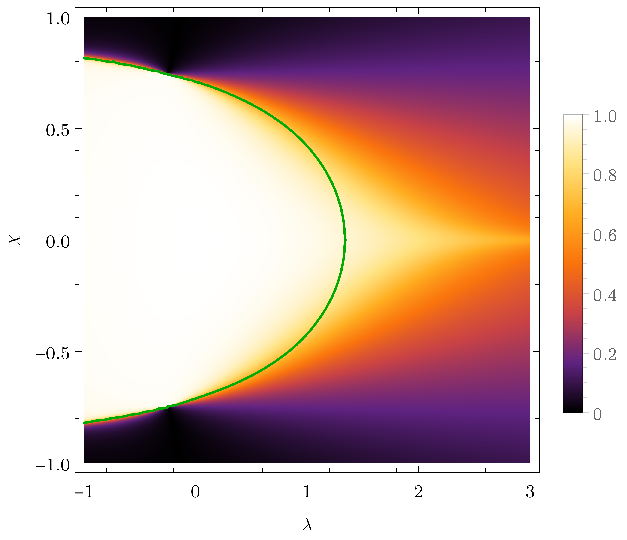
\includegraphics[scale=1.2]{../img/quenchFidelityFrom00.pdf}
    \caption{Arctangens of the fidelity of quench from $(\lambda_i;\chi_i)=(0;0)$ to the coordinate $(\lambda;\chi)$.}
    \label{fig:quenchFidelityFrom00}    
\end{figure}

% \begin{figure}[H]
%     \centering
%     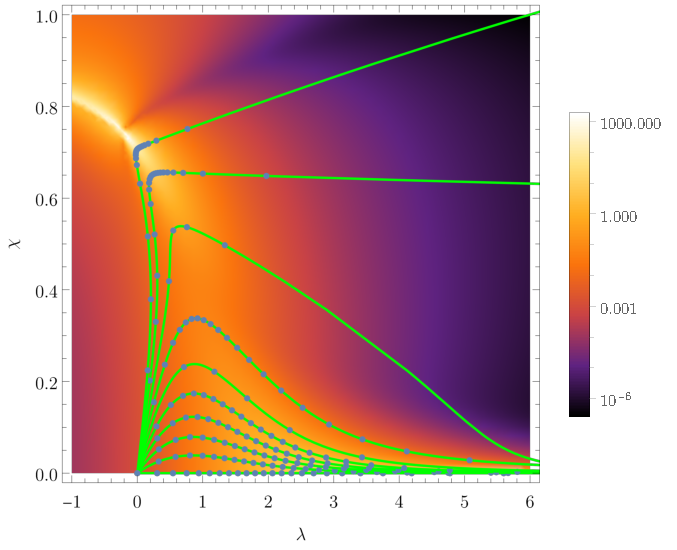
\includegraphics[scale=1.2]{../img/equidistantPointsOnPath.pdf}
%     \caption{Equidistant points on geodesics of the ground state manifold.}
%     \label{fig:equidistantPointsOnPath}    
% \end{figure}

\begin{figure}[H]
    \centering
    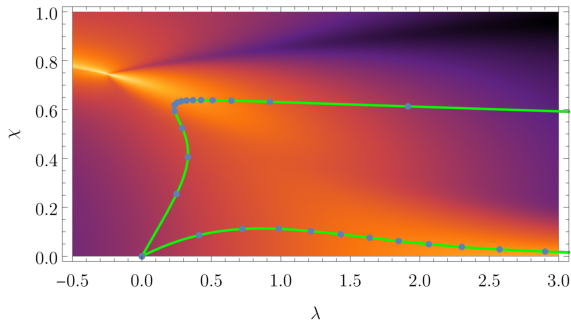
\includegraphics[scale=1.2]{../img/bg123.pdf}
    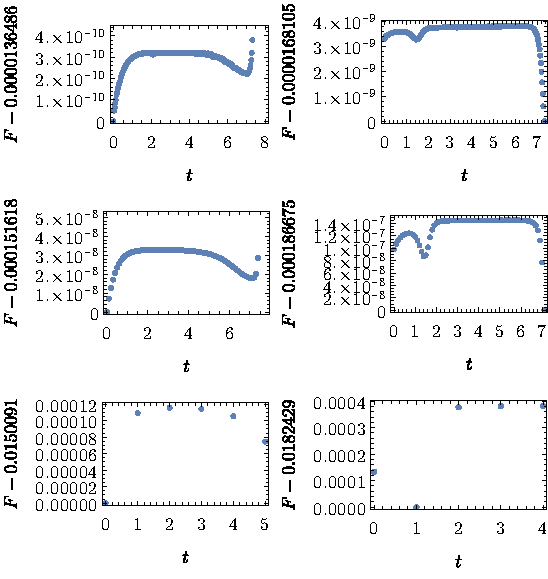
\includegraphics[scale=0.6]{../img/plotsFidelityQuenches.pdf}
    \caption{Fidelity for sequential quenches along geodesics (see green lines on top). Left (right) column corresponds to lower (upper) geodesic. Time steps from top are $\Delta t\in \{0.03,0.1,0.5\}$. Time difference between points in the plot on top is $\Delta t=0.5$.}
    \label{fig:plotsFidelityQuenches}    
\end{figure}


